\chapter{Conceitos e tecnologias estudadas}

\section{Problemas de Valor Inicial}
São os problemas nos quais são dados:
\begin{itemize}
  \item um conjunto de pontos iniciais $P$;
  \item o valor de $f(P_{0})$ para cada $P_{0} \in P$;
  \item um sistema de uma ou mais EDOs em $f$;
  \item e um tamanho de passo $h$.
\end{itemize}

Por fim, desejamos obter $f(P_{0} + h)$.

\section{Método de Integração Numérica Runge-Kutta}\label{rungekutta}
É um dos métodos para resolução de Problemas de Valor Inicial através da obtenção de uma aproximação para o valor de $f(P_{0} + h)$. Ele é uma generalização do Método de Euler através da aplicação de séries de Taylor (\ref{numerical-recipes}). Essa generalização nos permite a obtenção de diversas ordens do método, dentre as quais as mais comuns são 2 e 4, conhecidos como \textit{RK2} (ou, também, \textit{método do ponto médio}) e \textit{RK4}.

Ambos os métodos possuem termos da ordem de uma potência de $h$. Estes termos são o erro associado ao método e, portanto, quanto menor o tamanho do passo, menor o erro do método.

Logo, dado um Problema de Valor Inicial conforme descrito acima com uma única equação diferencial $g = f'$, temos os seguintes métodos definidos para apenas um ponto inicial, embora sua generalização para mais pontos consista apenas de sucessivas aplicações do mesmo método para cada ponto.

  \newpage
  \subsection{Ordem 2}
  Sejam $k_{1}$ e $k_{2}$ variáveis auxiliares, temos a seguinte expressão para o método de ordem 2:
  \newline
  \newline
  $k_{1} = h\ldotp g(P_{0})$\\
  $k_{2} = h\ldotp g(P_{0} + \frac{k_{1}}{2})$\\
  $f(P_{0} + h) = f(P_{0}) + k_{2} + O(h^{3})$
  
  \subsection{Ordem 4}
  Sejam $k_{1}$, $k_{2}$, $k_{3}$ e $k_{4}$ variáveis auxiliares, temos a seguinte expressão para o método de ordem 4:
  \newline
  \newline
  $k_{1} = h\ldotp g(P_{0})$\\
  $k_{2} = h\ldotp g(P_{0} + \frac{k_{1}}{2})$\\
  $k_{3} = h\ldotp g(P_{0} + \frac{k_{2}}{2})$\\
  $k_{4} = h\ldotp g(P_{0} + k_{3})$\\
  $f(P_{0} + h) = f(P_{0}) + \frac{k_{1}}{6} + \frac{k_{2}}{3} + \frac{k_{3}}{3} + \frac{k_{4}}{6} + O(h^{5})$

\section{Campo vetorial como discretização de EDOs}
Se calcularmos o valor de cada EDO em um conjunto finito de pontos $P$ obteremos então um campo vetorial que pode ser compreendido como a discretização destas equações neste conjunto limitado.
  \subsection{Algoritmos de aproximação}\label{aproximacao}
  Porém esta discretização exige uma aproximação para o caso onde desejamos obter um o valor da equação, em um ponto não definido no campo vetorial.

  \label{exemplo-campo}Como, por exemplo, o caso onde as coordenadas de todos os pontos são inteiros e o ponto desejado e alguma de suas coordenadas ao invés de ser inteira é um racional.

    \subsubsection{Nearest Neighbour}
    No caso do exemplo acima (\ref{exemplo-campo}), este algoritmo simplesmente aproxima o ponto desejado para o ponto mais próximo a este que esteja definido no campo vetorial.

    Ou seja, um algoritmo para uma das coordenadas cujo valor pretendido seja $a$, que pode ser generalizado para as demais, é:
    
    \begin{enumerate}
      \item Se $(a - \lfloor a\rfloor) \geq  0.5$ então devolvemos o valor em $\lceil a\rceil$;
      \item Caso contrário, então devolvemos o valor de $\lfloor a\rfloor$.
    \end{enumerate}
    
    \newpage
    \subsubsection{Interpolação trilinear}
    Antes de definir a interpolação trilinear é preciso definir a \textbf{interpolação linear}. Na qual dados dois pontos, $P_{1}$ e $P_{2}$, para os quais uma função $f$ está definida, o valor desta função em um ponto $P$, $f(P)$, sobre a reta $r$ que liga estes dois pontos é a ponderação do valor de $f(P_{1})$ e $f(P_{2})$ pela distância de $P$ a $P_{1}$ e $P_{2}$, respectivamente.
    
    Este método muito utilizado no $\Re ^{2}$ é dado por:
    
    $f(P) = f(P_{1}) + \frac{(f(P_{2}) - f(P_{1}))}{(P_{2} - P_{1})}\ldotp (P - P_{1})$
    
    Por sua vez a interpolação trilinear é inerentemente utilizada no $\Re ^{3}$. Ela pondera os oito pontos $P_{1}$, $P_{2}$, $P_{3}$, $P_{4}$, $P_{5}$, $P_{6}$, $P_{7}$ e $P_{8}$ definidos no campo para então obter $P$.
    
    No caso do exemplo \ref{exemplo-campo}, podemos compreender estes quatro pontos como os vértices do cubo que contém o ponto de interesse.
    
    \begin{figure}[!h]
      \begin{center}
         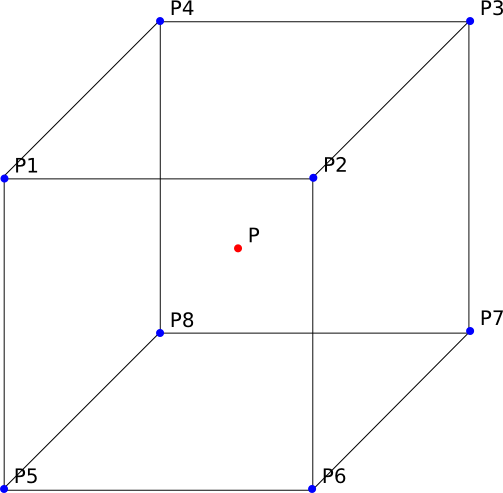
\includegraphics[width=60mm, height=60mm]{images/trilinearinterpolation.png}
         \label{fig:trilinearinterpolation}
         \caption{Os pontos cujas coordenadas são todas as combinações de chãos e tetos do ponto $P$ formam um cubo unitário que o contém}
      \end{center}
    \end{figure}
     
    A idéia do algoritmo é interpolar os pontos de cada aresta dois a dois na mesma coordenada sucessivamente. Se interpolarmos sobre $x$, depois sobre $y$ e por fim sobre $z$ para obtermos $P$, teremos as seguintes interpolações a serem calculadas:
    
    \newpage
    \begin{enumerate}
      \item $X_{1} = intp(P_{1}, P_{2})$;
      \item $X_{2} = intp(P_{3}, P_{4})$;
      \item $X_{3} = intp(P_{5}, P_{6})$;
      \item $X_{4} = intp(P_{7}, P_{8})$;
      \item $Y_{1} = intp(X_{1}, X_{2})$;
      \item $Y_{2} = intp(X_{3}, X_{4})$;
      \item $P = intp(Y_{1}, Y_{2})$.
    \end{enumerate}
    
    Onde $intp(A,B)$ é uma função que calcula a interpolação linear de $A$ e $B$.

\section{Computação de propósito geral na unidade de processamento gráfico}
\label{gpgpu}
Mais conhecida como \textit{General-Purpose computing on Graphics Processing Units (GPGPU)}, trata-se de  criar trechos de código que são executados na unidade de processamento gráfico ao invés de fazê-lo na \textit{CPU}. Este recurso é interessante para algoritmos altamente paralelizáveis uma vez que as unidades de processamento gráfico foram feitas para isto.

Por exemplo, uma NVIDIA GeForce GTX 690 possui mais de 3000 núcleos de processamento (\textit{CUDA Cores}) a aproximadamente 900MHz cada e 4GB de memória dedicada (\ref{gtx690}). O que representa um pequeno \textit{mainframe} à disposição para a execução de algoritmos paralelos. 

Ainda no princípio das placas gráficas dedicadas, percebendo seu poder computacional, teve início a programação de algoritmos gerais (isto é, algoritmos que não sejam de processamento gráfico) em termos de operações gráficas. Ou seja, os algoritmos eram traduzidos em termos multiplicações de matrizes para poderem ser processados na placa gráfica.

Com o crescimento deste tipo de uso, surgiu a linguagem \textit{Cg} facilitando a confecção de programas para a placa gráfica, mas que no fim das contas era compilado em termos de \textit{DirectX} ou \textit{OpenGL shaders}. Ou seja, ainda era apenas uma abstração para o processamento gráfico.

O que enfim levou a criação de linguagens de mais alto nível como \textit{OpenCL} e \textit{CUDA} que, do ponto de vista do programador, funcionam como uma extensão para linguagens como \textit{C}, \textit{C++}, \textit{Fortran} etc. Permitindo que quase não haja distinção entre programar para \textit{GPU} ou \textit{CPU}.

Antes de apresentar os detalhes das linguagens, é preciso destacar específicidades da programação para GPU que ainda não foram abstrataídas:

\begin{itemize}
  \item O trecho de código executado na \textit{GPU} é chamado de \textit{kernel}. Cada instância deste é chamada de \textit{thread}. Um conjunto de threads pode ser agrupado no que a NVIDIA chama de \textit{bloco}. E, por sua vez, estes podem ser agrupados no que a NVIDIA chama de \textit{grade};
  \item Os dados sobre os quais os algoritmos vão operar precisam ser transferidos da memória principal à memória dedicada da placa gráfica, através do barramento, e o resultado de volta. Esta transferência pode ser muito lenta, pois além do próprio barramento ser um gargalo, este ainda é compartilhado com todos os demais periféricos. Portanto, o primeiro objetivo é minimizar estas transferências a apenas o necessário e, quando elas forem necessárias, que sejam feitas em grandes quantidades de dados para usar toda a banda;
  \item Os diversos núcleos de processamento da unidade de processamento gráfico na verdade estão fisicamente agrupados no que é chamado de \textit{stream multiprocessors} pela NVIDIA. Isto é importante, pois todas as \textit{threads} de um bloco devem ser executadas no mesmo \textit{stream multiprocessor}. Ou seja, para utilizar toda capacidade da placa gráfica, é preciso ter vários \textit{blocos};
  \item A placa gráfica possui diferentes níveis de memória. A memória local contém as variáveis locais da thread, a memória compartilhada é a de acesso mais rápido para leitura, por estar dentro de cada \textit{stream multiprocessor}, e por fim a memória global. Para tornar o acesso à memória o menos custoso possível, é preciso fazer uso da memória compartilhada, embora o seu uso sem os devidos cuidados pode gerar erros de inconsistência semelhantes aos que podem ser vistos em um cache mal implementado. Ou seja, a escrita deve ser cuidadosa.
\end{itemize}
  \subsection{Linguagem CUDA}
  Atualmente na versão 4.2, é classificada como uma arquitetura para computação de propósito geral em paralelo introduzida em 2006 pela NVIDIA. Do ponto de vista do programador é uma extensão disponível para as linguagens \textit{C}, \textit{C++} e \textit{FORTRAN}. Os principais elementos do \textit{CUDA} são a hierarquia de agrupamento das threads, os níveis de memória e as barreiras de sincronização.
  
  A hierarquia de agrupamento consiste de dois níveis: grades (\textit{grids}) e blocos (\textit{blocks}). Um bloco agrupa muitas threads e uma grade, por sua vez, agrupa muitos blocos. Além de os blocos afetarem diretamente o escalonamento como descrito em \ref{gpgpu}, cada bloco possui um limite de threads que pode conter e o mesmo para grades com relação a blocos (este limite depende do hardware). Outro uso interessante para este agrupamento, é organizar processamento sobre dados que possuem três dimensões.
  
  O primeiro nível de memória é a memória local de cada thread privada, depois a memória compartilhada de cada bloco e, por fim, a memória global acessível por todas as threads. A memória global persiste até que seja desalocada pelo programa, enquanto as demais persistem apenas enquanto suas estruturas existem. As memórias local da thread e compartilhada do bloco são as mais rápidas ao custo de seu escopo limitado.
    
  \subsection{Linguagem OpenCL}
  A linguagem \textit{Open Computing Language (OpenCL)} foi especificada pelo \textit{Khronos Group} \ref{khronos}, um consórcio de várias empresas como AMD, ARM, Intel, IBM, Apple e até mesmo a NVIDIA, dentre muitas outras. O \textit{OpenCL} diferencia-se de \textit{CUDA} por ser um padrão aberto e de propósito geral para programação paralela em sistemas heterogêneos, ou seja, uma vez que o código seja desenvolvido em \textit{OpenCL}, poderá ser executado em \textit{GPU} e \textit{CPU}.

  O OpenCL foi idealizado em um modelo de plataforma, isto é, uma camada de abstração do \textit{hardware} heterogêneo. Uma plataforma é composta por um hospedeiro (\textit{host}) e por mais dispositivos de computação (\textit{compute devices}), que por sua vez são formados por unidades de computação (\textit{compute units}). A comunicação entre um dispositivo e o hospedeiro ocorre através de uma fila de comandos (\textit{command-queue}), esta fila pode ser composta de comandos de tranferência de dados, sicronização e execução de \textit{kernels}.

  A estrutura hierárquica de agrupamento ocorre em dois níveis, contexto e grupo de trabalho, e é similar a estrutura adotada por \textit{CUDA}. Um contexto (\textit{context}) é constituído dos recursos que um \textit{kernel} utilizará na sua execução, como dispositivos e dados armazenados na memória. Já um grupo de trabalho (\textit{work-group}) é um conjunto de itens de trabalho \textit{(work-items)}, que são equivalentes às \textit{threads} de \textit{CUDA}.

  O primeiro nível de memória é a memória privada que pertence a cada item de trabalho, depois a memória local de cada grupo de trabalho que é compartilahada por todos os itens de trabalho. O próximo nível é a memória global ou constante que está contida em cada dispositivo de computação. O último nível de memória corresponde a memória do \textit{host}.


  
  \subsection{Biblioteca VTK}
